\section{Список опытных фактов}

	\begin{enumerate}
		\item Существует электрическое взаимодействие, обусловленное зарядами между телами.
		\item Заряды \index{Заряд} существуют двух знаков: положительные и~отрицательные. Заряды одного знака отталкиваются, разных~-- притягиваются.
		\item Сила взаимодействия между точечными зарядами (электрическая сила) \index{Сила!взаимодействия!между точечными зарядами} обратно пропорциональна квадрату расстояния между ними. \\
				Рассмотрим два точечных заряда $q_1$ и $q_2$. Тогда:
					$$F \prop q_1, \quad F \prop q_2, \quad F \prop \frac{1}{r^2}, \,\,\text{откуда}\,\, F \prop \frac{q_1q_2}{r^2}.$$
				\begin{figure}[!h]
					\centering
					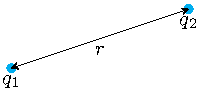
\includegraphics[scale=1.5]{./img/fig1/fig1.pdf}
					\caption{Два точечных заряда, $q_1$ и $q_2$}
				\end{figure}
		\item \textbf{[Закон Кулона]}\index{Закон!Кулона} В~системе СИ сила $F$ равна
				\begin{equation}\label{1}
					F=k\frac{q_1q_2}{r^2},
				\end{equation}
				где $k=9 \times 10^9 \,\dfrac{\text{H}\cdot \text{м}^2}{\text{Кл}^2}$, а $\dim{q}=\text{Кл (кулон)}$. \\
				Два единичных заряда на~расстоянии 1~м~будут взаимодействовать с~силой $F=9\times 10^9 \, \text{Н}$. Для измерения заряда те должны в~первую очередь сохраняться.
		\item \textbf{[Закон сохранения электрического заряда]} В замкнутой системе \index{Система!замкнутая} суммарный заряд сохраняется:
					$$q_{\Sigma}=\sum_i q_i=\c.$$
		\item \textbf{[Принцип суперпозиции]}\index{Принцип!суперпозиции} Сила, действующая на~данный электрический заряд $q$, равна векторной сумме всех сил, действующих в~системе:
				\begin{equation}\label{2}
					\vec{F} = \sum_i \vec{F}_i = \sum_i k\frac{qq_i\vec{r}_i}{r_i^3} \\
				\end{equation}
				\begin{figure}[!h]
					\centering
					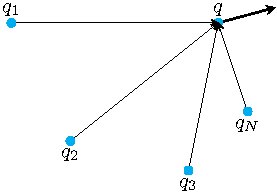
\includegraphics[scale=1.5]{./img/fig2/fig2.pdf}
					\caption{Система зарядов}
				\end{figure}
		\item \textbf{[Дискретность электрического заряда]}\index{Дискретность} Существует элементарный заряд $\bar{e}=1,6 \times 10^{-19} \, \text{Кл}$. Заряд любой частицы является кратным элементарному:
					$$q=n\bar{e}, \quad n \in \mathbb{Z}.$$
					Заряд электрона равен $q_{\text{эл}}=-\bar{e}$, протона $q_{\text{пр}}=+\bar{e}$.
	\end{enumerate}